\documentclass[master,euler,twoside,openright]{ustcthesis}% twoside 双面打印
% bachelor, doctor or master
% adobefont

% 设置图形文件的搜索路径
\graphicspath{{figures/}}

%仅用于本示例文档中显示特殊字符串
\usepackage{xltxtra}

\begin{document}


%%%%%%%%%%%%%%%%%%%%%%%%%%%%%%
%% 封面部分
%%%%%%%%%%%%%%%%%%%%%%%%%%%%%%

  % 中文封面内容
  \title{中国科学技术大学\\本硕博毕业论文模板\\示例文档(Beta)}%一般情况下扉页和书脊共用一个标题文本,可以不用定义\spinetitle。特殊情况见下。
  \spinetitle{\small{中国科学技术大学本硕博毕业论文模板示例文档\raisebox{-3pt}{(Beta)}}}
  %特殊情况1:本例中\title命令里含有换行控制字符,这回导致制作书脊的时候出现错误,例如如果你注释掉这一行就会报错。这时需要定义一个不含换行等命令的\spinetitle,这并不表示\spinetitle里不能有任何命令——只能使用有限的命令。
  %特殊情况2:本例中标题过长,所以需要缩小书脊标题的字号。
  %特殊情况3:本例中中英文混排,由于tex竖排的原理限制,中英文基线不重合,所以需要人工调整英文的基线。具体调整量根据不同字体有所不同。
  \author{赵\ 钱\ 孙}
  \depart{一二三系}%系别,硕博请用系代号,本科请用全称如
  %\depart{数理化和信息工程系}
  \major{人文管理和生物专业专业}%专业,硕博请用全称,本科不需要
  \advisor{周武正\ 教授}
  \coadvisor{冯晨珠\ 教授}%第二导师,没有请注释掉
  \submitdate{二〇九九年十三月}

  % 英文封面内容
  \entitle{USTC Thesis Template for Bachelor, Master and Doctor\\User's Guide(Beta)}
  \enauthor{Qiansun Zhao}
  \enmajor{Whatever}
  \enadvisor{Prof. Wuzheng Zhou}
  \encoadvisor{Prof. Chenzhu Feng}%另外一个导师
  \ensubmitdate{Thimber, 2099}

  % 封面
  \maketitle

%特别注意,以下属顺序为准,在对应部分添加文档部件,切勿颠倒顺序:
%本科论文的文档部件顺序是:
%    frontmatter:致谢、目录、中文摘要、英文摘要、
%    mainmatter: 正文章节
%    backmatter: 参考文献或资料注释、附录
%硕博论文的文档部件顺序是:
%    frontmatter:中文摘要、英文摘要、目录、符号说明
%    mainmatter: 正文章节
%    backmatter: 参考文献、附录、致谢、发表论文
%%%%%%%%%%%%%%%%%%%%%%%%%%%%%%
%% 前言部分
%%%%%%%%%%%%%%%%%%%%%%%%%%%%%%
\frontmatter
\makeatletter
\ifustc@bachelor
	%%%%%%%%%%%%%%%%%
	%本科论文修改这里
	%%%%%%%%%%%%%%%%%
	% 致谢
	\include{chapter/thanks}
	
	%目录部分
	%目录
	\tableofcontents
	%默认表格、插图、算法索引名称分别为“表格索引”、“插图索引”和“算法索引”
	%如果需要自行修改lot,lof,loa的名称,请定义
	%\ustclotname{...}
	%\ustclofname{...}
	%\ustcloaname{...}

	% 表格索引
	\ustclot
	% 插图索引
	\ustclof
	%算法索引 
	%如果需要使用算法环境并列出算法索引,请加入补充宏包。
	\ustcloa
	
	% 摘要
	\include{chapter/abstract}%此文件中含有中英文摘要
\else
	%%%%%%%%%%%%%%%%%
	%硕博论文修改这里
	%%%%%%%%%%%%%%%%%
	% 摘要
	\include{chapter/abstract}%此文件中含有中英文摘要
	% 目录
	\tableofcontents
	%默认表格、插图、算法索引名称分别为“表格索引”、“插图索引”和“算法索引”
	%如果需要自行修改lot,lof,loa的名称,请定义
	%\ustclotname{...}
	%\ustclofname{...}
	%\ustcloaname{...}

	% 表格索引
	\ustclot
	% 插图索引
	\ustclof
	%算法索引 
	%如果需要使用算法环境并列出算法索引,请加入补充宏包。
	%\ustcloa
	
	%符号说明,需要加入补充包
	\include{chapter/denotation}%不是必需的,如果不想列出请注释掉
\fi
\makeatother

%%%%%%%%%%%%%%%%%%%%%%%%%%%%%%
%% 正文部分
%%%%%%%%%%%%%%%%%%%%%%%%%%%%%%
\mainmatter


\chapter{标题}
\sanhao{标题}

  
\chapter{绪论}
\label{chap:introduction}

中国科学技术大学论文模板(ustcthesis)是按照中国科学技术大学学士、硕士和博士论文要求制作的\LaTeX 通用论文模板。其前身是中国科学技术大学本科论文模板(作者XPS,最后维护ywg)和中国科学技术大学研究生论文模板(作者Liuqs,主要维护Liuqs、Guolicai)。本模板在上述两模板基础上进行了整合梳理,将模板的基础实现和增强功能进行分离,分别提供最基础的ustcthesis.cls以及增强包ustcxtra.cls。其中,ustcthesis.cls仅提供模板的最基础格式,ustcxtra.cls则包含一些常用的优化设置及更为便捷的自定义命令。

本文是使用上述模板生成的示例文档,目的在于帮助使用者熟悉该模板的使用方法,并且为使用者学位论文的撰写提供基础代码示例。

\section{系统要求}
\subsection{系统要求}
本模板基于\CTeX 的ctexbook文档类进行定制,基于\XeTeX 引擎排版。使用本模板的最基础功能时,除了上述需求外,还需要如下几类宏包(直接引用):
\begin{description}
\item[数学类]{amsmath、amsthm、amsfonts、amssymb、bm}
\item[格式类]{titletoc、titlesec、geometry}
\item[表格类]{multicol、multirow}
\item[其他]{xeCJK、hyperref、natbib}
\end{description}
可能有部分宏包是由上述宏包以及\CTeX 间接引用的,此处不一一列举。

另外,如果需要使用增强的ustcxtra.cls,额外需要如下宏包(直接引用):
\begin{description}
\item[默认载入]{times、algorithm2e、graphicx、psfrag、subfig、enumerate、epsfig、float、paralist、booktabs、footmisc、wasysym、longtable、bbm、indentfirst、ifthen、caption3、array、fancyvrb、xcolor、url}
\item[条件载入]{eulervm(仅在文档类处于增强模式并在文档类选项注明euler时载入)}
\end{description}

\section{下载与安装}
\subsection{模板文件清单}
使用模板之前请确保模板文件没有缺失损坏。文件清单如\autoref{tab:filelist},标注关键的文件需要确保文件以及路径的完整。
\begin{table}[htp]
\centering
\tabcaption{模板文件清单}
\label{tab:filelist}
\begin{tabular}{lll}
\toprule
文件名&相对路径&备注\tabularnewline
\midrule
clean.bat			&./			&清理脚本\tabularnewline
clean.sh			&./			&清理脚本\tabularnewline
main.pdf			&./			&示例文件\tabularnewline
main.tex 			&./			&示例TeX文件\tabularnewline
make.bat			&./			&生成脚本\tabularnewline
make.sh				&./			&生成脚本\tabularnewline
readme.txt			&./			&关于\tabularnewline
ustcbib.bst		&./			&Bib格式文件\tabularnewline
ustcthesis.cls		&./			&(关键)模板\tabularnewline
ustcxtra.cls		&./			&(关键)模板增强\tabularnewline
ustc\_logo\_fig.eps	&./figures	&(关键)科大校徽\tabularnewline
ustc\_logo\_text.eps&./figures	&(关键)科大校名\tabularnewline
\bottomrule
\end{tabular}
\end{table}

\subsection{模板下载与使用}
本模板及本示例文件可以在Google Project网站\url{http://code.google.com/p/ustcthesis}下载。备份托管地址为\url{https://gitlab.lug.ustc.edu.cn/ywg/ustcthesis},此托管网站由LUG@USTC提供服务

\textbf{特别注意:}由于Google在2014年之后停止了新建下载的功能,目前在Google Code网站不能在Download页面找到下载链接。请通过“source”页面->选择“default”Repository->点击“browse”->download “zip”来下载最新的模板(见\autoref{fig:download})。也可以通过git clone的方式获得模板。

\begin{figure}
\centering
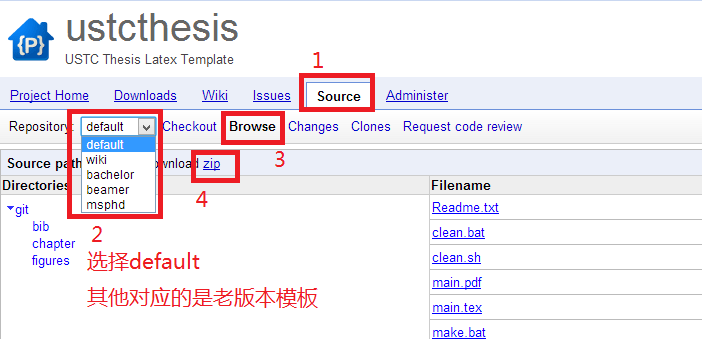
\includegraphics[width=0.9\textwidth]{download}
\figcaption{在Google Code上进行模板下载}
\label{fig:download}
\end{figure}

\textbf{特别注意2:}此前开发的本科和硕博模板已暂停支持,但仍然可以通过在download页面中通过搜索功能查找并下载,也可以在source中选择对应的Repository进行下载。

模板的安装使用方法有多种,最为简单便捷的方法是直接解压缩下载好的压缩包,修改其中的main.tex文件以及chapter文件夹下的文件,必要时增加所需要的文件。需要注意的是确保所有文件使用UTF-8编码。Windows系统中将其他编码的文件转化为UTF-8的方法是: 用记事本打开这些文件, 然后点击文件—另存为—在最下方选择UTF-8 编码。

\subsection{\texorpdfstring{\LaTeX}{LaTeX}系统的安装和使用}
由于本模板使用了较多的宏包,因此建议使用TeXLive2013及以上版本的\LaTeX 发行版。TeXLive2013可以在Windows、GNU/Linux和大多数Unix系统中运行。对于MacOSX,推荐使用MacTeX-2013。详细信息参考\url{https://www.tug.org/texlive/}。

对于中国科学技术大学的校内用户而言,最方便的获取TeXLive2013的途径是使用LUG@USTC提供的CTAN镜像源(\url{http://mirrors.ustc.edu.cn/CTAN/})。最新的TeXLive位于/CTAN/systems/texlive/目录(\url{http://mirrors.ustc.edu.cn/CTAN/systems/texlive/})内。用户可以选择进入Images文件夹下载完整的光盘并刻录安装,也可以选择进入tlnet文件夹下载运行install-tl.exe进行在线安装。需要注意的是,在线安装的时候可以通过切换安装源为本校镜像源来加快下载安装速度。

对于校外用户,可以通过CTAN.org获得官方的TeXLive。CTAN在全球41个国家和地区分布有115个镜像站点,它们的地址可以在\url{http://www.ctan.org/mirrors/}找到。

\subsection{推荐使用的编辑器}
\LaTeX 的源文件是一个或多个文本文件,这意味着可以使用最为简单的文本编辑器来撰写论文。但是和许多编程语言类似,使用一款带有语法高亮、命令补全等功能的文本编辑器能够大大提升协作效率。

对于不同的编辑器而言,能够实现的功能也不尽相同,加之不同用户拥有不同的使用习惯,简单武断的说某一款编辑器好或者不好有失公允。对于\TeX 写作而言,用户使用的编辑器大致可以分为两类:通用的文本编辑器和专用的GUI编辑器。通用的文本编辑器中公认比较好用的有Vim(Linux)、Emacs(Linux)、Notepad++(Windows)等等\footnote{当然,这些软件可能都有跨平台版本,而且也有其他很多优秀的文本编辑器,不要在意这些细节啦,我并不想挑起编辑器的圣战。:P}。这些编辑器有着强大的功能,但是往往需要在编辑和编译之间来回切换。而专用的GUI编辑器如TeXShop(Mac)、TeXWorks(windows/Linux)和Winedit(Windows、付费软件)等虽然可能在文本编辑上略显笨拙,但是其优点在于编写和生成一体化,简单化。

使用何种编辑器这个问题见仁见智,但是对于一个刚从word转来的新人,从界面简洁、操作简单、功能实用的角度出发,TeXWorks不失为一款优秀的GUI软件,如\autoref{fig:texworks}。

\begin{figure}
\centering
\includegraphics[width=0.9\textwidth]{texworks}
\figcaption{TeXWorks主界面}
\label{fig:texworks}
\end{figure}

Windows系统下TeXWorks的界面拥有左右两个窗口,左边为编辑窗口,右边为预览窗口,当编辑完文档之后,只需点击绿色的开始按钮,就可以立即对文档进行保存并编译,可以选择不同的引擎进行处理。编译过程中的信息会在左侧窗口下方显示。TeXWorks默认UTF-8编码,安装时自动查找TeX安装目录,支持自动缩进、语法高亮、命令补全、正则式查找以及TeX文件和PDF的正反查找(即点击命令跳转到对应pdf文字位置以及点击pdf文字跳转到对应命令,操作是Ctrl+单击)。这些功能对新手来说都是十分友好的。

\section{问题反馈}

如果您在使用过程中有疑问,遇到困难,可以在\href{http://bbs.ustc.edu.cn/cgi/bbsdoc?board=TeX}{瀚海星云\TeX{}讨论区}或者相关的\LaTeX 论坛(如\href{http://bbs.ctex.org}{CTEX 论坛})寻求帮助,但是请注意遵守论坛的各项规定。

如果使用过程中遇到Bug,请提交到\href{http://bbs.ustc.edu.cn/cgi/bbsdoc?board=TeX}{瀚海星云\TeX{}讨论区},或者提交到相应的\href{http://code.google.com/p/ustcthesis/issues/list}{Google UstcThesis Project(http://code.google.com/p/ustcthesis/issues/list)},请注明是什么版本模板的bug。
  \chapter{模板的基础使用说明}

\section{模板基本说明}
使用本模板,您应首先具备基本的\LaTeX 知识,如果您刚刚接触\LaTeX,建议您先学习相关的用户文档或教程。

模板文件名为ustcthesis.cls。方便起见,将该文件放置在与论文主文件同一文件夹中即可。如果需要使用增强功能,模板提供了一个名为ustcxtra.cls的补充包。将该文件放置在与论文主文件同一文件夹中即可。

模板提供一个文档类ustcthesis,使用\verb|\documentclass{ustcthesis}|来加载模板。

模板可以使用ctexbook文档类的相应选项,默认加载的是 cs4size, a4paper, fancyhdr, fntef。需要注意的是默认加载 \emph{双面/章节从奇数页开始} 选项,如果需要\emph{单面} 选项,请使用:
\begin{Code}
\documentclass[<学位>,oneside,openany]{ustcthesis}
\end{Code}

\begin{table}[htp]
\centering
\tabcaption{模板提供的新文档选项}
\label{tab:newdocopt}
\begin{tabular}{lL{5cm}L{4cm}}
\toprule
文档选项&说明&备注\tabularnewline
\midrule
bachelor	&学士				&\multirow{3}{4cm}{指明论文类型,不能同时存在}\tabularnewline
master		&硕士				&\tabularnewline
doctor		&博士				&\tabularnewline
basic		&仅使用基础功能	&此时无法使用增强包中的命令\tabularnewline
oldfontcfg	&使用老版本的硕博论文模板的字体设置			&需要补充包\tabularnewline
euler		&使用euler数学字体&需要补充包\tabularnewline
adobefont	&使用adobe的字体	&\multirow{2}{4cm}{仅仅防止误输入}\tabularnewline
adobefonts	&使用adobe的字体	&\tabularnewline
\bottomrule
\end{tabular}
\end{table}

\subsection{模板推荐加载设置}
推荐使用如下选项加载模板:
\begin{Code}
\documentclass[<学位>,euler,twoside,openright]{ustcthesis}
\end{Code}

如果缺少大多数宏包,建议使用
\begin{Code}
\documentclass[<学位>,basic,twoside,openright]{ustcthesis}
\end{Code}

\section{模板提供的新环境和命令}
模板提供了若干个新环境和命令,如\autoref{tab:newenv}和\autoref{tab:newcmd}所列,这些新环境和命令有的比较简单,有的则附有对应的示例。

\begin{longtable}{lll}%@{\extracolsep{\fill}}
\caption[模板提供的新环境]{模板提供的新环境}
\label{tab:newenv} \\
\toprule
名称  & 说明 & 备注\tabularnewline\midrule
\endfirsthead
\bottomrule
\endfoot
\caption[模板提供的新环境(续)]{模板提供的新环境(续)} 
\label{tab:newenv2} \\
\toprule
名称  & 说明 & 备注\tabularnewline\midrule
\endhead
\bottomrule
\endlastfoot
enabstract&英文摘要&\tabularnewline
cnabstract&中文摘要&\tabularnewline
thanks&致谢&\tabularnewline
denotation&主要符号对照表&需要ustcxtra,用法见./chapter/denotation.tex\tabularnewline
Code&代码&需要ustcxtra,效果见\autoref{codex}\tabularnewline
Codex&代码&需要ustcxtra,效果见\autoref{codex}\tabularnewline
CodeScript&代码&需要ustcxtra,效果见\autoref{codex}\tabularnewline
CodexScript&代码&需要ustcxtra,效果见\autoref{codex}\tabularnewline
code&代码&需要ustcxtra,效果未测试\tabularnewline
theorem &定理&\tabularnewline
lemma &引理&\tabularnewline
example &例&\tabularnewline
algorithm &算法&\tabularnewline
definition &定义& \tabularnewline
axiom &公理 &\tabularnewline
property &性质 & \tabularnewline
proposition &命题 &\tabularnewline
corollary& 推论 &\tabularnewline
remark &注解  &\tabularnewline
condition &条件 & \tabularnewline
conclusion &结论 & \tabularnewline
assumption &假设 & \tabularnewline
prove &证明 &\tabularnewline
proof&证明 &与prove的区别见\autoref{pic:proofandprove}\tabularnewline
\end{longtable}

\begin{longtable}{lll}%@{\extracolsep{\fill}}
\caption[模板提供的新命令]{模板提供的新命令}
\label{tab:newcmd} \\
\toprule
名称  & 说明 & 备注\tabularnewline\midrule
\endfirsthead
\bottomrule
\endfoot
\caption[模板提供的主要新命令(续)]{模板提供的主要新命令(续)} 
\label{tab:newcmd2} \\
\toprule
名称  & 说明 & 备注\tabularnewline\midrule
\endhead
\bottomrule
\endlastfoot
\textbackslash chuhao\{\}&字号:初号&类似的有:\textbackslash yihao\{\}...\textbackslash qihao\{\}\tabularnewline
\textbackslash xiaochu\{\}&字号:小初号&类似的有:\textbackslash xiaoer\{\}...\textbackslash xiaowu\{\}\tabularnewline
\textbackslash xiaochuhao\{\}&字号:小初号&类似的有:\textbackslash xiaoerhao\{\}...\textbackslash xiaowuhao\{\}\tabularnewline
\textbackslash ustclofname\{\}&定义图表索引名称&需在\textbackslash ustclof前使用\tabularnewline
\textbackslash ustclof&生成图表索引并加入目录&\tabularnewline
\textbackslash ustclotname\{\}&表格索引名称&与\textbackslash ustclofname\{\}类似\tabularnewline
\textbackslash ustclot&表格索引&与\textbackslash ustclot类似\tabularnewline
\textbackslash ustcloaname\{\}&算法索引名称&需要ustcxtra,与\textbackslash ustclofname\{\}类似\tabularnewline
\textbackslash ustcloa&算法索引&需要ustcxtra,与\textbackslash ustclof类似\tabularnewline
\textbackslash title\{\}&标题&中文\tabularnewline
\textbackslash author\{\}&作者&中文\tabularnewline
\textbackslash advisor\{\}&导师&中文\tabularnewline
\textbackslash coadvisor\{\}&第二导师&中文,可留空\tabularnewline
\textbackslash major\{\}&专业&硕博全称,本科不需要\tabularnewline
\textbackslash depart\{\}&院系&硕博代号,本科全称\tabularnewline
\textbackslash submitdate\{\}&完成日期&中文\tabularnewline
\textbackslash en...\{\}&由title至submitdate&以上命令的英文版本\tabularnewline
\textbackslash studentid\{\}&学号&仅本科需要\tabularnewline
\textbackslash spinetitle\{\}&书脊使用的标题&在\textbackslash title中含有部分控制命令时使用\tabularnewline
\textbackslash keywords\{\}&中文关键词&在cnabstract中使用\tabularnewline
\textbackslash enkeywords\{\}&英文关键词&在enabstract中使用\tabularnewline
\textbackslash figcaption\{\}&图形标题&无论是否在图形环境中均可得到正确标题\tabularnewline
\textbackslash tabcaption\{\}&&与上类似,表格用\tabularnewline
C\{width\}&定宽居中&表格环境中p\{width\}的加强,参考\autoref{tab:tblcmp}\tabularnewline
L\{width\}&定宽左齐&\tabularnewline
R\{width\}&定宽右齐&\tabularnewline
\textbackslash scite\{\}&上标引用&\tabularnewline
\textbackslash song&宋体&另有其他,详见ustcxtra\tabularnewline
\textbackslash upGamma&立直希腊Gamma&另有其他,详见ustcxtra\tabularnewline
\end{longtable}

需要注意的是,这里prove环境翻译为“证明”,事实上,其实prove环境不是用作theorem等类似环境配套证明的,prove环境是与theorem等环境同级别的环境。与theorem等环境相配套的证明环境是proof环境。使用时请注意下两个环境的差异:proof环境是没有编号的,是与theorem这类环境配合使用的;prove环境是有编号的,更多的是类似于证明题的题目。详细的差别见\autoref{pic:proofandprove}。

\begin{figure}
\centering
  \framebox{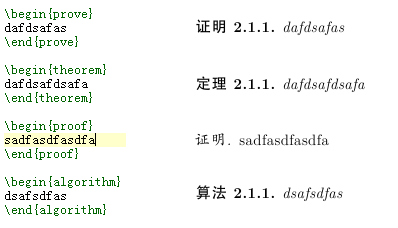
\includegraphics[scale=1]{figures/proofandprove}}
  \figcaption{proof、prove以及部分其他数学环境的差异}
  \label{pic:proofandprove}
\end{figure}

\section{使用模板的一些建议}

公式、章节、图和表格等(不包括脚注和参考文献)的交叉引用可以使用\verb|\autoref{label}|来得到正确的引用。例如使用\verb|\autoref{some_pic}|可以得到“图 X”的引用,使用\verb|\autoref{some_table}|可以得到“表 X”的引用。

建议使用\verb|\figcaption{}|命令得到所有图形的标题,表格也是。这样无论是否在图形环境中均能够得到正确的带图/表编号的标题,而在图形环境之外使用\verb|\caption{}|命令会报错。

%封面是按照制本厂的要求制作的,其中行宽和行高都是固定的,中文标题最多占两行,英文标题最多占三行。如果您的题目超过了这个限制,请缩减题目长度,不要擅自修改模板中的相关配置参数。


  \include{chapter/chap-example}
  %自行添加
  %\include{chapter/...}

  %参考文献测试:\citep{knuth86e}


%%%%%%%%%%%%%%%%%%%%%%%%%%%%%%
%% 附件部分
%%%%%%%%%%%%%%%%%%%%%%%%%%%%%%
\backmatter

  % 参考文献
  % 使用 BibTeX
  % 选择参考文献的排版格式。注意ustcbib这个格式不保证完全符合要求,请自行决定是否使用
  \bibliographystyle{ustcbib}%{GBT7714-2005NLang-UTF8}
  \bibliography{bib/tex}
  \nocite{*} % for every item
  % 不使用 BibTeX
  % \include{chapter/bib}

  % 附录,没有请注释掉
  \begin{appendix}
    
\chapter{关于硕士、博士学位论文撰写要求}
\label{chap:requires}

学位论文是学位申请者为申请学位而撰写的学术论文,它集中作者在研究工作中获得可行的发明、理论和见解,是评判学位申请人学术水平的重要依据和获得学位的必要条件之一,也是科研领域中的主要文献资料和社会宝贵财富。
为提高研究生学位论文的质量,做到学位论文在内容和格式上规范化与统一化,特作如下规定:

\section{对学位论文的基本要求}

\textbf{一下文字仅作示例,一切以学校规定为准!}

\subsection{硕士学位论文}

根据《中华人民共和国学位条例暂行实施办法》第八条的规定,硕士学位论文应能表明作者确已在本门学科上掌握了坚实的基础理论和系统的专门知识,并对所研究的课题有新的见解,有从事科学研究或独立担负专门技术工作的能力。硕士学位论文工作一般是在硕士生完成培养计划规定的课程学习后开始,其工作内容因学科的性质不同而有所差异,一般包括文献阅读、开题报告、拟定并实施工作计划、科研调查、实验研究、理论分析和文字总结等工作。论文正文一般应不少于3万字。硕士学位论文必须有一定的工作量,在论文题目确定后,用于论文工作的时间一般不应少于1.5年。

\subsection{博士学位论文}

根据《中华人民共和国学位条例暂行实施办法》第十三条的规定,博士学位论文应能表明作者确已在本门学科上掌握了坚实宽广的基础理论和系统深入的专门知识,具有独立从事科学研究工作的能力,并在科学或专门技术工作上做出了创造性的成果。博士学位论文工作是攻读博士学位研究生培养的最重要环节,其工作时间一般应不少于2学年。博士生入学后在导师指导下明确科研方向,收集资料,阅读文献,进行调查研究,确定研究课题。一般在第二至第三学期通过开题报告并制定论文工作计划。博士生应根据论文工作计划分阶段在教研室、学术会议上报告科研和论文工作的进展情况。论文正文一般应不少于5万字。博士生用于论文研究和撰写学位论文的时间一般应不得少于2年。

特别应注意,学位论文应是本人的研究成果,在导师指导下独立完成,不得抄袭或剽窃他人成果。论文应反映作者较好地掌握了本学科、专业的研究方法和技能,学术观点必须言之有理、持之有据,论文内容应层次分明,数据可靠,文字简炼,推理严谨,立论正确。

\section{对学位论文的格式要求}

\subsection{编写要求}

硕士、博士学位论文一般应由以下全部或某几部分组成,依次为:封面、中文摘要、英文摘要 、目录、符号说明、正文、参考文献、附录、附图表、致谢、攻读学位期间发表的学术论文目录。

具体要求如下:

\subsubsection{封面}

采用研究生院规定的统一封面,封面上填写论文题目、作者姓名、导师姓名、学科(专业) 、论文完成时间。上述内容也应在扉页上填写清楚。论文题目采用黑体26磅加粗居中,其他采用宋体16磅居中。书脊用黑体12磅,上方写论文题目,中间写系别,下方写研究生姓名(彩色封面在制信厂或印刷厂装订)。

\subsubsection{论文摘要}

学位论文的中文摘要应以最简洁的语言介绍论文的概要、作者的突出论点、新见解或创造性成果。硕士学位论文中文摘要一般应在500字左右,博士学位论文中文摘要一般在1500字左右。英文摘要(Abstract)内容应与中文摘要基本相对应,要语句通顺,语法正确,能正确概括文章的内容。摘要标题采用黑体16磅居中,正文采用宋体12磅(英文用Times New Roman体12磅),行距20磅。

\subsubsection{正文}

正文是学位论文的主体和核心部分,它是将学习、研究和调查过程中筛选、观察和测试所获得的材料,经过加工整理和分析研究,由材料而形成论点。不同学科、专业有着不同的写作内容,但作为一般要求,论据、论点应力求准确、完备、清晰、通顺,实事求是,客观真切,简短精炼,合乎逻辑。一般标题字体采用黑体14磅,多级标题可采用粗体14磅或粗体12磅。正文字体采用宋体12磅(英文用Times New Roman体12磅),两端对齐书写,行距20磅。


绪论或引言是学位论文主体部分的开端,主要说明研究工作的缘起、沿革、目的、涉及范围 、国内外研究现状、相关领域的前人研究成果和知识空白、理论分析的依据、研究设想、研究方法和实际设计的概述,以及文中拟解决的问题、理论意义和实用价值等,应言简意赅,不要与摘要雷同或成为摘要的解释,也不是提要。

结论是学位论文最终和总体的结论,是整篇论文的归宿,应明确、精炼、完整、准确。要着重阐述作者研究的创造性成果、新见解、新发现和新发展,及其在本研究领域中的地位、作用、价值和意义,还可进一步提出需要讨论的问题和建议。学位论文中的计量单位、制图、制表、公式规范、缩略词和符号必须遵循GB 3100~3102—93(国家技术监督局1993-12-27发布,1994-07-01实施)有关量和单位的规定。如无标准可循,应采用本学科或专业有关权威性机构或学术团体所公布的规定。如不得已必需引用某些未公知公用的、不易为同行读者所理解的或系作者自行拟定的符合、记号、缩略词等,均应一一在第一次出现时加以说明,给以明确的定义。

\subsubsection{参考文献}

参考文献应按文中引用的顺序列出,可以分列在各章末尾,也可以列在正文的末尾。

本着以严谨求实的科学态度撰写论文,凡学位论文中有引用他人成果之处,均应详细列出所引文献的名称、作者、发表刊物、发表时间、卷号、页码等。标题字体采用黑体14磅,正文字体采用宋体10磅(英文用Times New Roman体10磅),行距16磅。

\subsubsection{附录}
主要列入正文内过分冗长的公式推导,供查读方便所需的辅助性数学工具或表格,重复性数据图表,论文使用的缩写,程序全文及说明等。

\subsubsection{致谢}

表达作者对完成论文和学业提供帮助的老师、同学、领导、同事及亲属的感激之情。

\subsubsection{攻读学位期间发表的学术论文目录}

按学术论文发表的时间顺序,列齐本人在攻读学位期间发表或已录用的学术论文清单(发表刊物名称、卷册号、页码、年月及论文署名、作者排序)。

\subsection{打印}

按照有关规定,凡授予中华人民共和国学位者,学位论文必须用中文撰写,同时一律用A4标准纸打印输出,一般应有篇眉。篇眉和页码均采用宋体10磅居中,页面设置上边距3.8cm、下边距为3.0cm,左边距为3.5cm、右边距为3.0cm。

\subsection{装订}

学位论文撰写完成后,用研究生院统一封面线装订成册。所需份数由研究生本人及导师掌握(可参考学位申请上报材料清单的要求)。

  \end{appendix}

  \makeatletter
  \ifustc@bachelor\relax\else
    % 致谢
	\include{chapter/thanks}%硕博致谢部分
    % 发表文章目录
    \include{chapter/pub}
  \fi
  \makeatother

  

\end{document}
